\documentclass{article}

\usepackage{graphicx}
\usepackage{geometry}
\geometry{
    a4paper,
    total={170mm,257mm},
    left=20mm,
    top=20mm,
}

\begin{document}

% \fbox{
\begin{figure}[h!]
    \begin{minipage}{0.5\textwidth}
        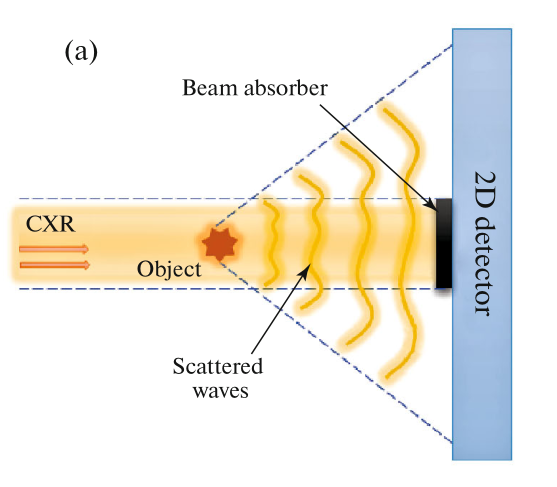
\includegraphics[width=\textwidth]{plane_wave_approximation.png}
        \caption{CDI in plane wave approximation}
    \end{minipage}%
    \begin{minipage}{0.5\textwidth}
        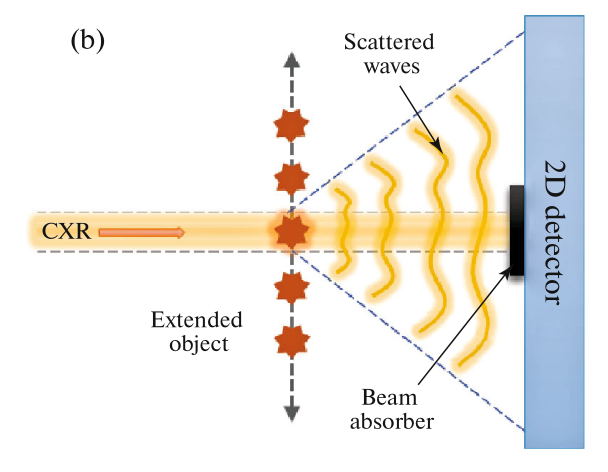
\includegraphics[width=\textwidth]{ptychography.png}
        \caption{X-ray ptychography}
    \end{minipage}

    \begin{minipage}{0.5\textwidth}
        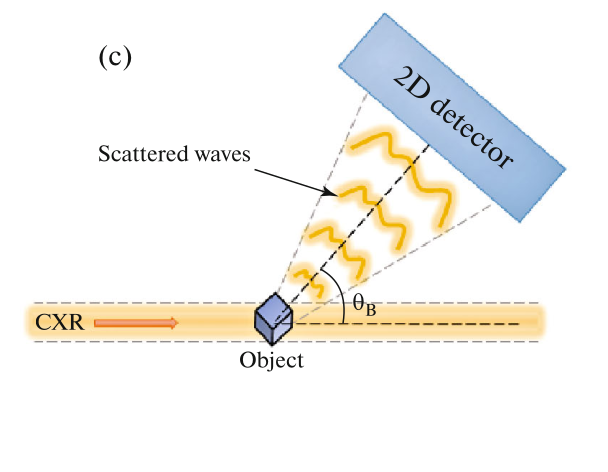
\includegraphics[width=\textwidth]{braggs-geometryy.png}
        \caption{CDI in Bragg geometry}
    \end{minipage}%
    \begin{minipage}{0.5\textwidth}
        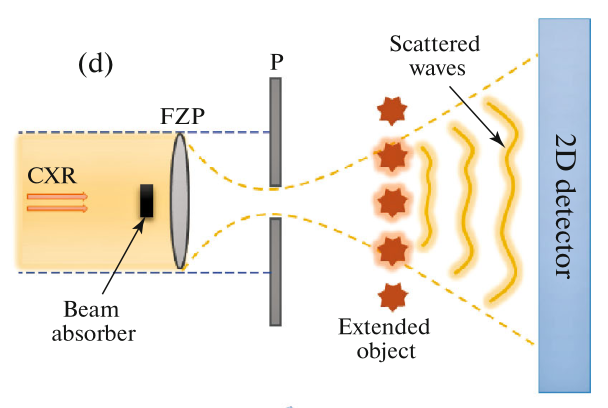
\includegraphics[width=\textwidth]{Fresnel approximation.png}
        \caption{Fresnel approximation}
    \end{minipage}

    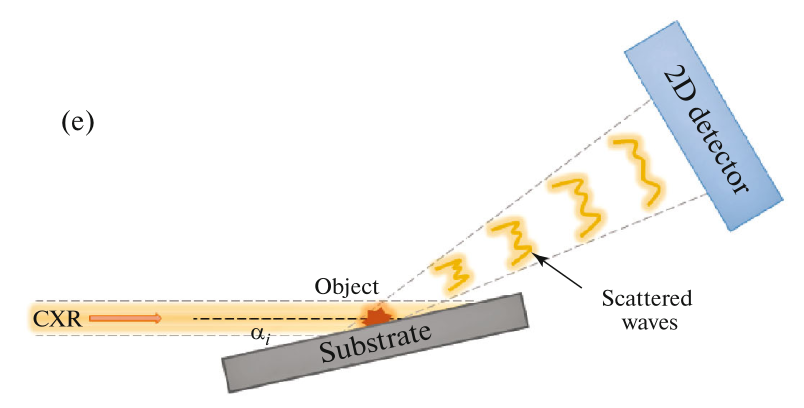
\includegraphics[width=\textwidth]{TER_geometry.png}
    \caption{CDI in TIR}
\end{figure}
% }


\end{document}